\documentclass[12pt]{article}

\usepackage{sbc-template}

\usepackage{graphicx,url}

%\usepackage[brazil]{babel}
\usepackage[latin1]{inputenc}


\sloppy

\title{Tabela de Simbolos \\ Compiladores}

\author{ Arthur C�mara \\ Guilherme Cordeiro }


\address{Universidade Federal De Minas Gerais}

\begin{document}

\maketitle

\section{ Decis�es de Projeto: }

A decis�o de projeto mais relevante para esta etapa foi escolher implementa��o da tabela de simbolos por meio de hash. Esta escolhe � feita pois apresenta um bom desempenho se comparada as demais implementa��es.

\section{ C�digo }

O c�digo foi retirado do site. A estrutura foi encapsulada em uma classe de c++ para facilitar os trabalhos futuros. Utilizamos a assinatura de m�todos j� implementada.
Uma pequena teste foi realizado para comprovar o funcionamento da Tabela de Simbolos. Neste teste, executamos diversas a��es sobre a tabela para verificar se todos os conceitos estavam de acordo.

\begin{figure}[ht]
\centering
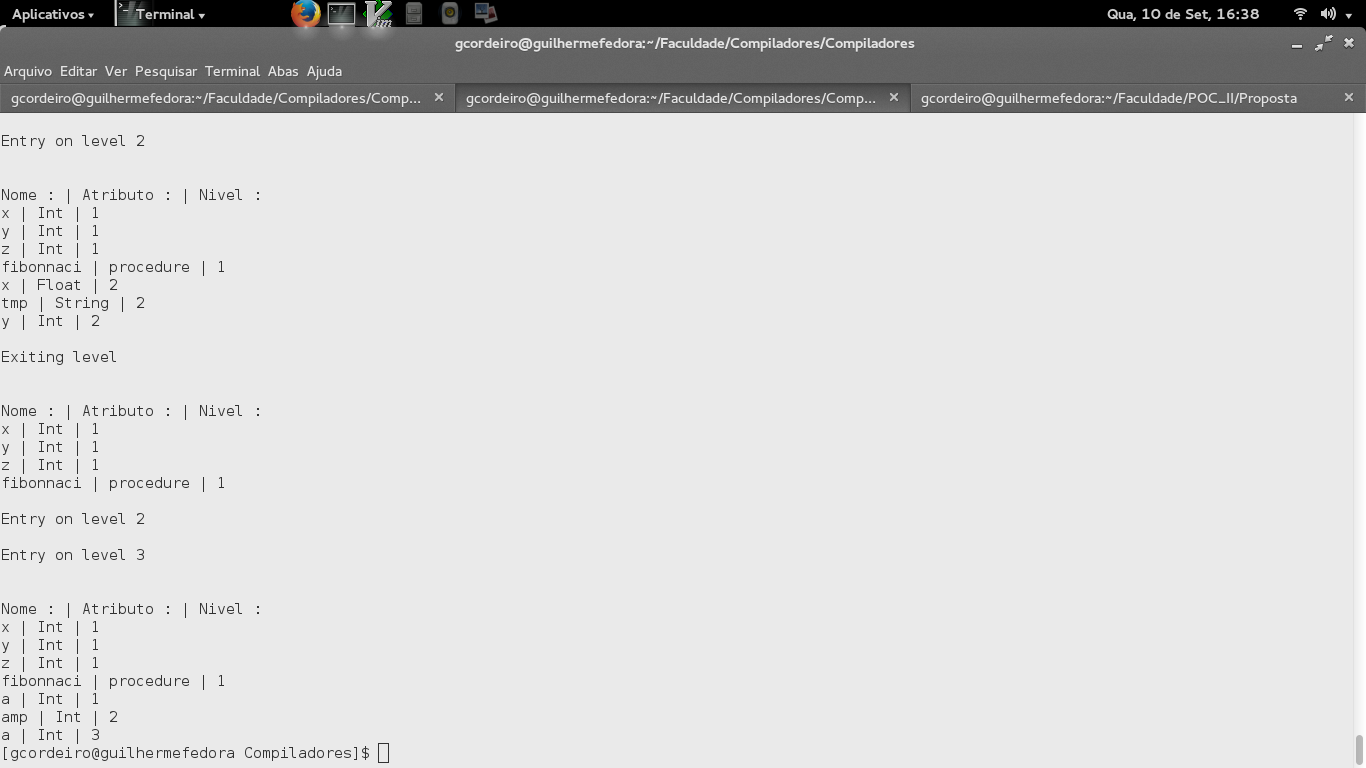
\includegraphics[width=1\textwidth]{teste.png}
\caption{Execu��o da Tabela de Simbolos}
\label{fig:exampleFig1}
\end{figure}

Neste teste, mostramos entrada e sa�da de blocos e recupera��o dos simbolos da tabela.





\end{document}
